\documentclass[]{article}
\usepackage{lmodern}
\usepackage{amssymb,amsmath}
\usepackage{ifxetex,ifluatex}
\usepackage{fixltx2e} % provides \textsubscript
\ifnum 0\ifxetex 1\fi\ifluatex 1\fi=0 % if pdftex
  \usepackage[T1]{fontenc}
  \usepackage[utf8]{inputenc}
\else % if luatex or xelatex
  \ifxetex
    \usepackage{mathspec}
  \else
    \usepackage{fontspec}
  \fi
  \defaultfontfeatures{Ligatures=TeX,Scale=MatchLowercase}
\fi
% use upquote if available, for straight quotes in verbatim environments
\IfFileExists{upquote.sty}{\usepackage{upquote}}{}
% use microtype if available
\IfFileExists{microtype.sty}{%
\usepackage{microtype}
\UseMicrotypeSet[protrusion]{basicmath} % disable protrusion for tt fonts
}{}
\usepackage[margin=1in]{geometry}
\usepackage{hyperref}
\hypersetup{unicode=true,
            pdftitle={ggtree},
            pdfauthor={Suraj Bhattarai},
            pdfborder={0 0 0},
            breaklinks=true}
\urlstyle{same}  % don't use monospace font for urls
\usepackage{color}
\usepackage{fancyvrb}
\newcommand{\VerbBar}{|}
\newcommand{\VERB}{\Verb[commandchars=\\\{\}]}
\DefineVerbatimEnvironment{Highlighting}{Verbatim}{commandchars=\\\{\}}
% Add ',fontsize=\small' for more characters per line
\usepackage{framed}
\definecolor{shadecolor}{RGB}{248,248,248}
\newenvironment{Shaded}{\begin{snugshade}}{\end{snugshade}}
\newcommand{\KeywordTok}[1]{\textcolor[rgb]{0.13,0.29,0.53}{\textbf{#1}}}
\newcommand{\DataTypeTok}[1]{\textcolor[rgb]{0.13,0.29,0.53}{#1}}
\newcommand{\DecValTok}[1]{\textcolor[rgb]{0.00,0.00,0.81}{#1}}
\newcommand{\BaseNTok}[1]{\textcolor[rgb]{0.00,0.00,0.81}{#1}}
\newcommand{\FloatTok}[1]{\textcolor[rgb]{0.00,0.00,0.81}{#1}}
\newcommand{\ConstantTok}[1]{\textcolor[rgb]{0.00,0.00,0.00}{#1}}
\newcommand{\CharTok}[1]{\textcolor[rgb]{0.31,0.60,0.02}{#1}}
\newcommand{\SpecialCharTok}[1]{\textcolor[rgb]{0.00,0.00,0.00}{#1}}
\newcommand{\StringTok}[1]{\textcolor[rgb]{0.31,0.60,0.02}{#1}}
\newcommand{\VerbatimStringTok}[1]{\textcolor[rgb]{0.31,0.60,0.02}{#1}}
\newcommand{\SpecialStringTok}[1]{\textcolor[rgb]{0.31,0.60,0.02}{#1}}
\newcommand{\ImportTok}[1]{#1}
\newcommand{\CommentTok}[1]{\textcolor[rgb]{0.56,0.35,0.01}{\textit{#1}}}
\newcommand{\DocumentationTok}[1]{\textcolor[rgb]{0.56,0.35,0.01}{\textbf{\textit{#1}}}}
\newcommand{\AnnotationTok}[1]{\textcolor[rgb]{0.56,0.35,0.01}{\textbf{\textit{#1}}}}
\newcommand{\CommentVarTok}[1]{\textcolor[rgb]{0.56,0.35,0.01}{\textbf{\textit{#1}}}}
\newcommand{\OtherTok}[1]{\textcolor[rgb]{0.56,0.35,0.01}{#1}}
\newcommand{\FunctionTok}[1]{\textcolor[rgb]{0.00,0.00,0.00}{#1}}
\newcommand{\VariableTok}[1]{\textcolor[rgb]{0.00,0.00,0.00}{#1}}
\newcommand{\ControlFlowTok}[1]{\textcolor[rgb]{0.13,0.29,0.53}{\textbf{#1}}}
\newcommand{\OperatorTok}[1]{\textcolor[rgb]{0.81,0.36,0.00}{\textbf{#1}}}
\newcommand{\BuiltInTok}[1]{#1}
\newcommand{\ExtensionTok}[1]{#1}
\newcommand{\PreprocessorTok}[1]{\textcolor[rgb]{0.56,0.35,0.01}{\textit{#1}}}
\newcommand{\AttributeTok}[1]{\textcolor[rgb]{0.77,0.63,0.00}{#1}}
\newcommand{\RegionMarkerTok}[1]{#1}
\newcommand{\InformationTok}[1]{\textcolor[rgb]{0.56,0.35,0.01}{\textbf{\textit{#1}}}}
\newcommand{\WarningTok}[1]{\textcolor[rgb]{0.56,0.35,0.01}{\textbf{\textit{#1}}}}
\newcommand{\AlertTok}[1]{\textcolor[rgb]{0.94,0.16,0.16}{#1}}
\newcommand{\ErrorTok}[1]{\textcolor[rgb]{0.64,0.00,0.00}{\textbf{#1}}}
\newcommand{\NormalTok}[1]{#1}
\usepackage{graphicx,grffile}
\makeatletter
\def\maxwidth{\ifdim\Gin@nat@width>\linewidth\linewidth\else\Gin@nat@width\fi}
\def\maxheight{\ifdim\Gin@nat@height>\textheight\textheight\else\Gin@nat@height\fi}
\makeatother
% Scale images if necessary, so that they will not overflow the page
% margins by default, and it is still possible to overwrite the defaults
% using explicit options in \includegraphics[width, height, ...]{}
\setkeys{Gin}{width=\maxwidth,height=\maxheight,keepaspectratio}
\IfFileExists{parskip.sty}{%
\usepackage{parskip}
}{% else
\setlength{\parindent}{0pt}
\setlength{\parskip}{6pt plus 2pt minus 1pt}
}
\setlength{\emergencystretch}{3em}  % prevent overfull lines
\providecommand{\tightlist}{%
  \setlength{\itemsep}{0pt}\setlength{\parskip}{0pt}}
\setcounter{secnumdepth}{0}
% Redefines (sub)paragraphs to behave more like sections
\ifx\paragraph\undefined\else
\let\oldparagraph\paragraph
\renewcommand{\paragraph}[1]{\oldparagraph{#1}\mbox{}}
\fi
\ifx\subparagraph\undefined\else
\let\oldsubparagraph\subparagraph
\renewcommand{\subparagraph}[1]{\oldsubparagraph{#1}\mbox{}}
\fi

%%% Use protect on footnotes to avoid problems with footnotes in titles
\let\rmarkdownfootnote\footnote%
\def\footnote{\protect\rmarkdownfootnote}

%%% Change title format to be more compact
\usepackage{titling}

% Create subtitle command for use in maketitle
\newcommand{\subtitle}[1]{
  \posttitle{
    \begin{center}\large#1\end{center}
    }
}

\setlength{\droptitle}{-2em}

  \title{ggtree}
    \pretitle{\vspace{\droptitle}\centering\huge}
  \posttitle{\par}
    \author{Suraj Bhattarai}
    \preauthor{\centering\large\emph}
  \postauthor{\par}
      \predate{\centering\large\emph}
  \postdate{\par}
    \date{November 27, 2018}


\begin{document}
\maketitle

\subsection{INTRODUCTION}\label{introduction}

R package for visualization and annotations of phylogenetic trees

\begin{itemize}
\tightlist
\item
  Designed by extending the \emph{ggplot2}.
\item
  Other R packages that implement tree viewer using \emph{ggplot2} are
  \textbf{OutbreakTools}, \textbf{phyloseq} and \textbf{ggphylo}.
\item
  These packages interpret phylogenetic as a collection of lines, which
  makes it hard to annotate diverse user input that are related to node
  (taxa).
\item
  The \emph{ggtree} is different to them by interpreting a tree as a
  collection of taxa and allowing general flexibilities of annotating
  phylogenetic tree with diverse types of user inputs.
\end{itemize}

\begin{Shaded}
\begin{Highlighting}[]
\KeywordTok{library}\NormalTok{(ggtree)}
\end{Highlighting}
\end{Shaded}

\begin{verbatim}
## ggtree v1.14.2  For help: https://guangchuangyu.github.io/software/ggtree
## 
## If you use ggtree in published research, please cite the most appropriate paper(s):
## 
## <U+25C9> Guangchuang Yu, David Smith, Huachen Zhu, Yi Guan, Tommy Tsan-Yuk Lam. ggtree: an R package for visualization and annotation of phylogenetic trees with their covariates and other associated data. Methods in Ecology and Evolution 2017, 8(1):28-36, doi:10.1111/2041-210X.12628
## 
## <U+25C9> Guangchuang Yu, Tommy Tsan-Yuk Lam, Huachen Zhu, Yi Guan. Two methods for mapping and visualizing associated data on phylogeny using ggtree. Molecular Biology and Evolution 2018, accepted. doi: 10.1093/molbev/msy194
\end{verbatim}

\begin{Shaded}
\begin{Highlighting}[]
\KeywordTok{library}\NormalTok{(ggplot2)}
\CommentTok{#library(treeio)}
\end{Highlighting}
\end{Shaded}

To view a phylogenetic tree, we first need to parse the tree file into
R. The ggtree (Yu et al. 2017) package supports many file formats via
the treeio package, including output files of commonly used software
packages in evolutionary biology.

\subsection{TREE VISUALIZATION}\label{tree-visualization}

\begin{Shaded}
\begin{Highlighting}[]
\KeywordTok{set.seed}\NormalTok{(}\DecValTok{11282018}\NormalTok{)}
\NormalTok{tree <-}\StringTok{ }\KeywordTok{rtree}\NormalTok{(}\DecValTok{50}\NormalTok{)}
\KeywordTok{ggtree}\NormalTok{(tree)}
\end{Highlighting}
\end{Shaded}

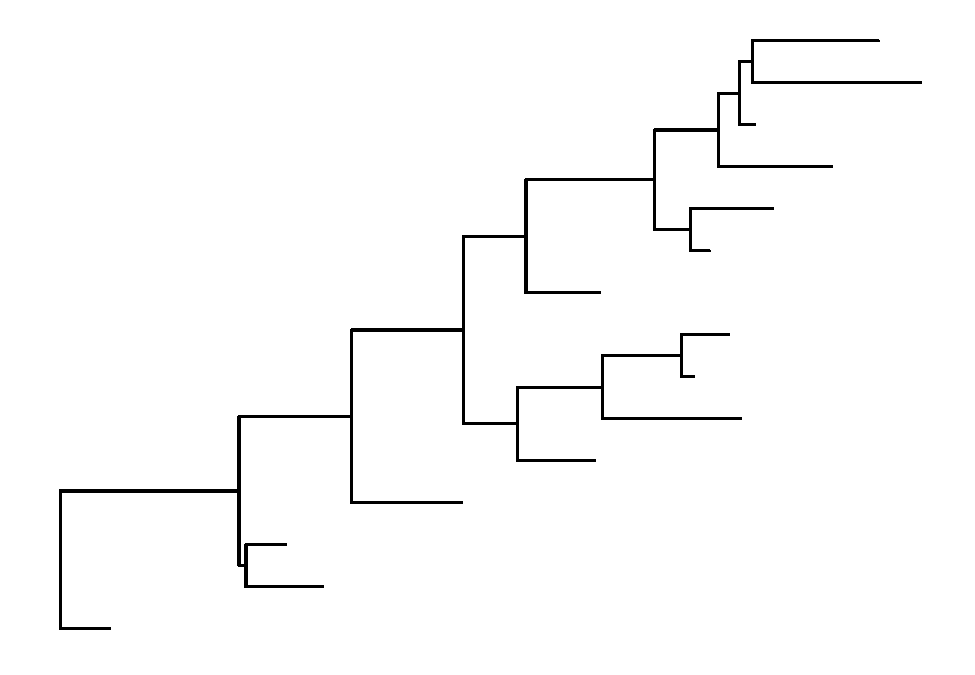
\includegraphics{ggtree_files/figure-latex/unnamed-chunk-2-1.pdf}

can use ggplot2 by implementing a geom\_tree layer

\begin{Shaded}
\begin{Highlighting}[]
\KeywordTok{ggplot}\NormalTok{(tree, }\KeywordTok{aes}\NormalTok{(x, y)) }\OperatorTok{+}\StringTok{ }\KeywordTok{geom_tree}\NormalTok{() }\OperatorTok{+}\StringTok{ }\KeywordTok{theme_tree}\NormalTok{()}
\end{Highlighting}
\end{Shaded}

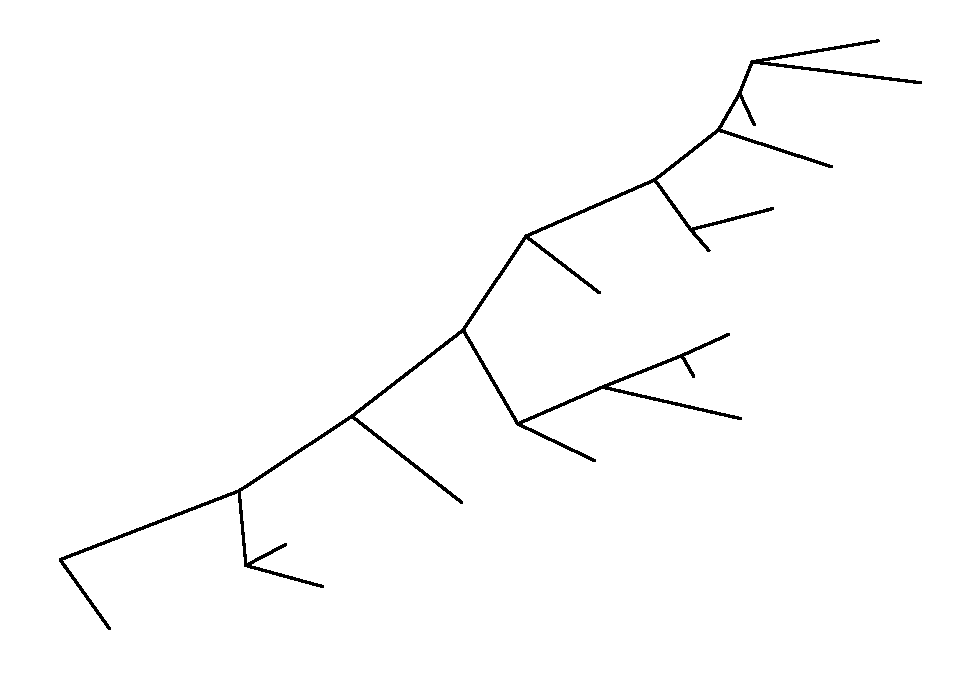
\includegraphics{ggtree_files/figure-latex/unnamed-chunk-3-1.pdf}

\subsubsection{Tree layout}\label{tree-layout}

Rectangular (by default) slanted circular fan

Phylogram and Cladogram (in phylogram branch length represents time)

\begin{Shaded}
\begin{Highlighting}[]
\KeywordTok{ggtree}\NormalTok{(tree, }\DataTypeTok{layout=}\StringTok{"slanted"}\NormalTok{) }\CommentTok{# phylogram}
\end{Highlighting}
\end{Shaded}

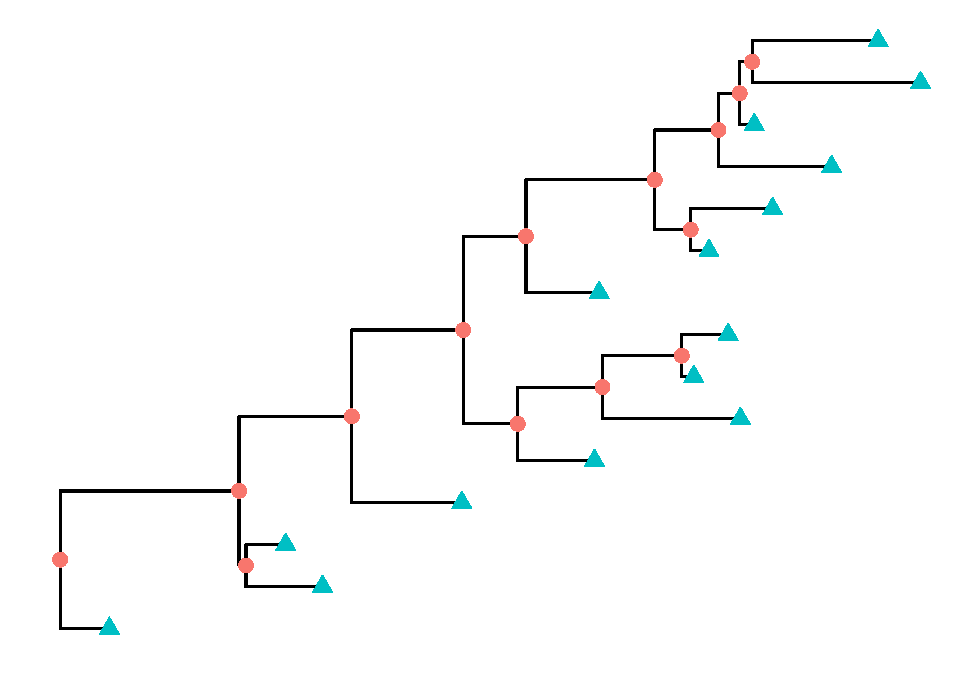
\includegraphics{ggtree_files/figure-latex/unnamed-chunk-4-1.pdf}

\begin{Shaded}
\begin{Highlighting}[]
\KeywordTok{ggtree}\NormalTok{(tree, }\DataTypeTok{layout=}\StringTok{"circular"}\NormalTok{) }\CommentTok{# phylogram}
\end{Highlighting}
\end{Shaded}

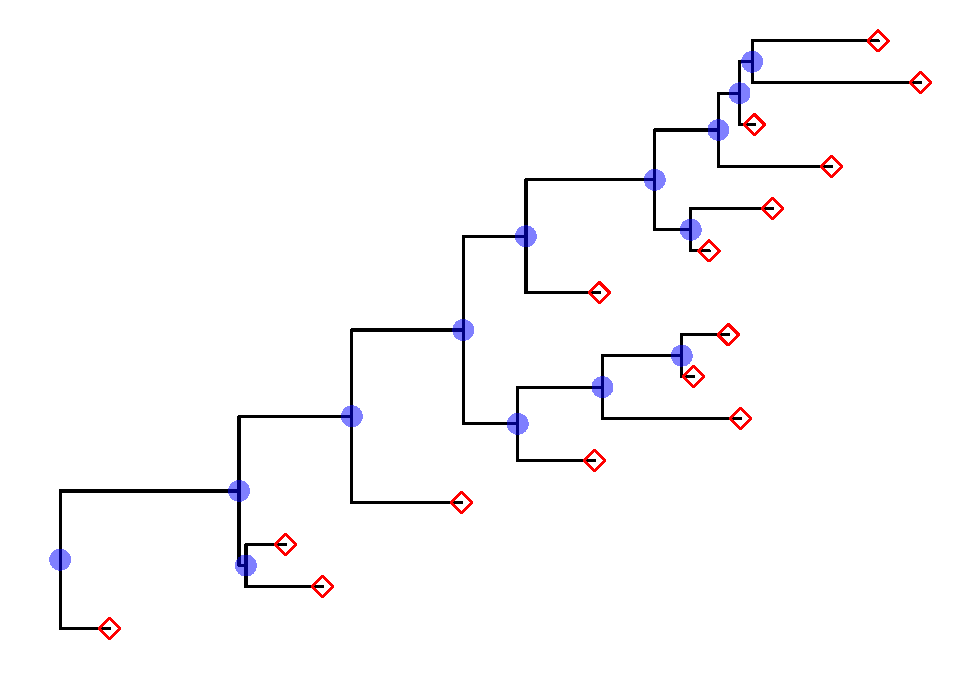
\includegraphics{ggtree_files/figure-latex/unnamed-chunk-4-2.pdf}

\begin{Shaded}
\begin{Highlighting}[]
\KeywordTok{ggtree}\NormalTok{(tree, }\DataTypeTok{layout=}\StringTok{"fan"}\NormalTok{, }\DataTypeTok{open.angle=}\DecValTok{120}\NormalTok{) }\CommentTok{# phylogram}
\end{Highlighting}
\end{Shaded}

\includegraphics{ggtree_files/figure-latex/unnamed-chunk-4-3.pdf}

\begin{Shaded}
\begin{Highlighting}[]
\KeywordTok{ggtree}\NormalTok{(tree, }\DataTypeTok{layout=}\StringTok{"equal_angle"}\NormalTok{) }\CommentTok{# unrooted}
\end{Highlighting}
\end{Shaded}

\includegraphics{ggtree_files/figure-latex/unnamed-chunk-4-4.pdf}

\begin{Shaded}
\begin{Highlighting}[]
\KeywordTok{ggtree}\NormalTok{(tree, }\DataTypeTok{layout=}\StringTok{"daylight"}\NormalTok{) }\CommentTok{# unrooted}
\end{Highlighting}
\end{Shaded}

\begin{verbatim}
## Average angle change [1] 0.133843760721467
\end{verbatim}

\begin{verbatim}
## Average angle change [2] 0.0530980905146852
\end{verbatim}

\begin{verbatim}
## Average angle change [3] 0.0309079136251543
\end{verbatim}

\includegraphics{ggtree_files/figure-latex/unnamed-chunk-4-5.pdf}

\begin{Shaded}
\begin{Highlighting}[]
\KeywordTok{ggtree}\NormalTok{(tree, }\DataTypeTok{branch.length=}\StringTok{'none'}\NormalTok{) }\CommentTok{# rectangular cladogram}
\end{Highlighting}
\end{Shaded}

\includegraphics{ggtree_files/figure-latex/unnamed-chunk-4-6.pdf}

\begin{Shaded}
\begin{Highlighting}[]
\KeywordTok{ggtree}\NormalTok{(tree, }\DataTypeTok{branch.length=}\StringTok{'none'}\NormalTok{, }\DataTypeTok{layout=}\StringTok{'circular'}\NormalTok{) }\CommentTok{# circular cladogram}
\end{Highlighting}
\end{Shaded}

\includegraphics{ggtree_files/figure-latex/unnamed-chunk-4-7.pdf}

\begin{Shaded}
\begin{Highlighting}[]
\KeywordTok{ggtree}\NormalTok{(tree, }\DataTypeTok{layout=}\StringTok{"daylight"}\NormalTok{, }\DataTypeTok{branch.length=}\StringTok{'none'}\NormalTok{) }\CommentTok{# daylight cladogram}
\end{Highlighting}
\end{Shaded}

\begin{verbatim}
## Average angle change [1] 0.133843760721467
\end{verbatim}

\begin{verbatim}
## Average angle change [2] 0.0530980905146852
\end{verbatim}

\begin{verbatim}
## Average angle change [3] 0.0309079136251543
\end{verbatim}

\includegraphics{ggtree_files/figure-latex/unnamed-chunk-4-8.pdf}

Displaying tree scale (evolution distance) using geom\_treescale layer

\begin{Shaded}
\begin{Highlighting}[]
\KeywordTok{ggtree}\NormalTok{(tree) }\OperatorTok{+}\StringTok{ }\KeywordTok{geom_treescale}\NormalTok{()}
\end{Highlighting}
\end{Shaded}

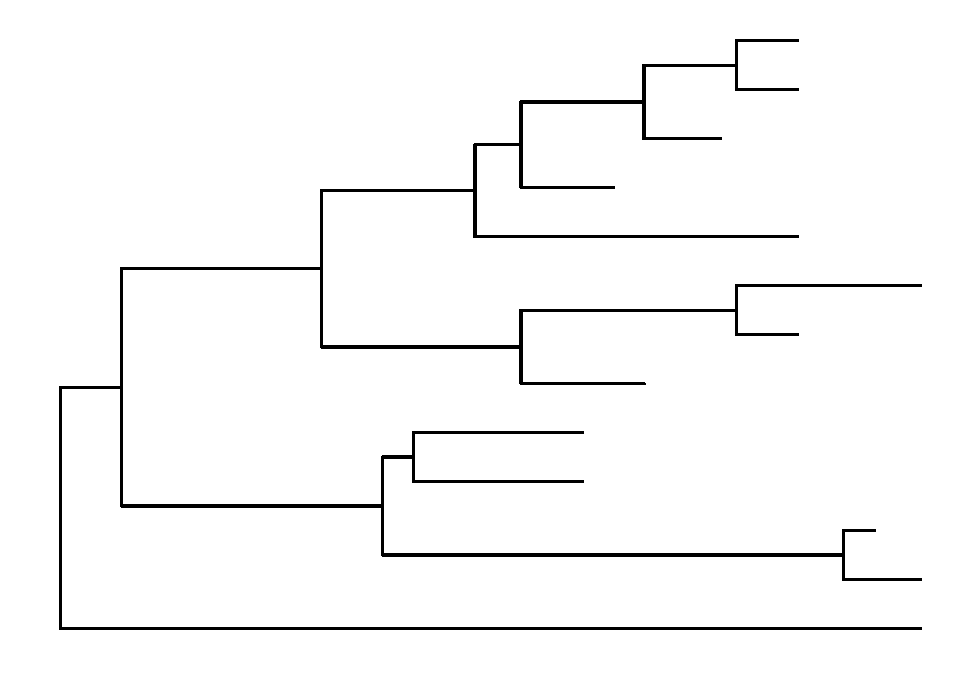
\includegraphics{ggtree_files/figure-latex/unnamed-chunk-5-1.pdf}

\subsubsection{Parameters in
geom\_treescale}\label{parameters-in-geom_treescale}

\begin{itemize}
\tightlist
\item
  x and y for tree scale position
\item
  width for the length of the tree scale
\item
  fontsize for the size of the text
\item
  linesize for the size of the line
\item
  offset for relative position of the line and the text
\item
  color for color of the tree scale
\end{itemize}

\begin{Shaded}
\begin{Highlighting}[]
\KeywordTok{ggtree}\NormalTok{(tree) }\OperatorTok{+}\StringTok{ }\KeywordTok{geom_treescale}\NormalTok{(}\DataTypeTok{x=}\DecValTok{0}\NormalTok{, }\DataTypeTok{y=}\DecValTok{12}\NormalTok{, }\DataTypeTok{width=}\DecValTok{6}\NormalTok{, }\DataTypeTok{color=}\StringTok{'red'}\NormalTok{)}
\end{Highlighting}
\end{Shaded}

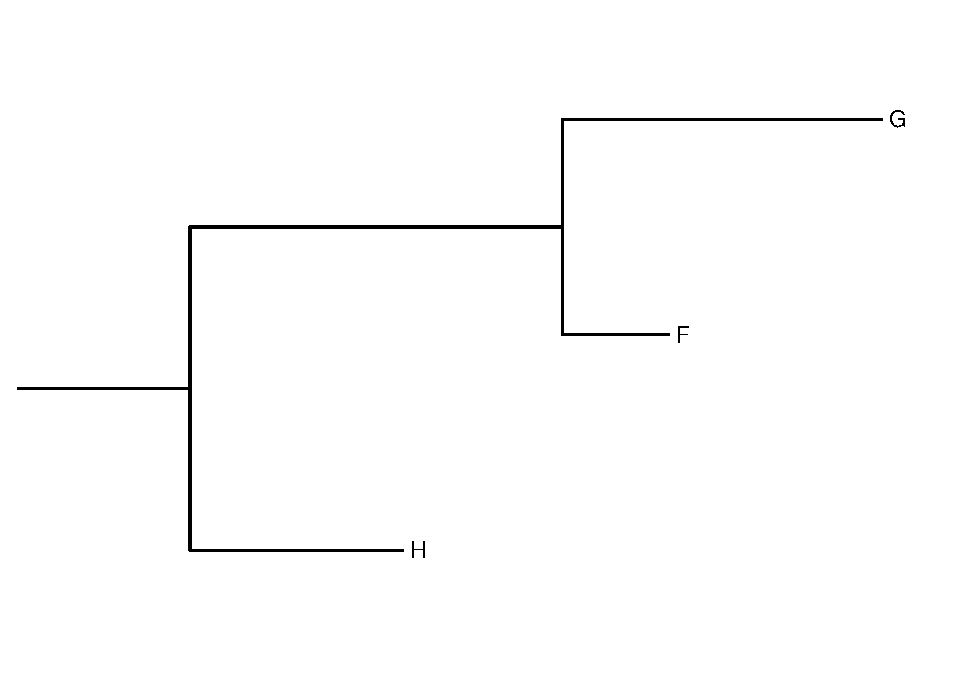
\includegraphics{ggtree_files/figure-latex/unnamed-chunk-6-1.pdf}

\begin{Shaded}
\begin{Highlighting}[]
\CommentTok{#ggtree(tree) + geom_treescale(x=0, y=0, width=4, color='red')}
\KeywordTok{ggtree}\NormalTok{(tree) }\OperatorTok{+}\StringTok{ }\KeywordTok{geom_treescale}\NormalTok{(}\DataTypeTok{fontsize=}\DecValTok{8}\NormalTok{, }\DataTypeTok{linesize=}\DecValTok{2}\NormalTok{, }\DataTypeTok{offset=}\OperatorTok{-}\DecValTok{1}\NormalTok{)}
\end{Highlighting}
\end{Shaded}

\includegraphics{ggtree_files/figure-latex/unnamed-chunk-6-2.pdf}

\subsubsection{Displaying nodes/ tips}\label{displaying-nodes-tips}

\begin{Shaded}
\begin{Highlighting}[]
\CommentTok{# use geom_nodepoint, geom_tippoint or geom_point}

\KeywordTok{ggtree}\NormalTok{(tree) }\OperatorTok{+}\StringTok{ }\KeywordTok{geom_point}\NormalTok{(}\KeywordTok{aes}\NormalTok{(}\DataTypeTok{shape=}\NormalTok{isTip, }\DataTypeTok{color=}\NormalTok{isTip), }\DataTypeTok{size=}\DecValTok{3}\NormalTok{)}
\end{Highlighting}
\end{Shaded}

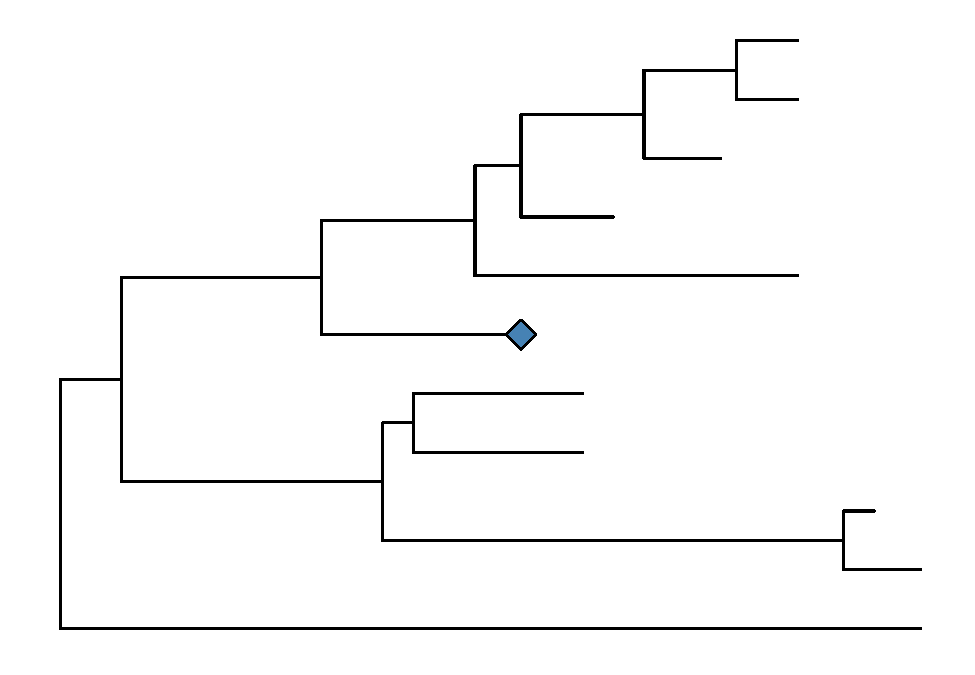
\includegraphics{ggtree_files/figure-latex/unnamed-chunk-7-1.pdf}

\begin{Shaded}
\begin{Highlighting}[]
\NormalTok{p <-}\StringTok{ }\KeywordTok{ggtree}\NormalTok{(tree) }\OperatorTok{+}\StringTok{ }\KeywordTok{geom_nodepoint}\NormalTok{(}\DataTypeTok{color=}\StringTok{"#b5e521"}\NormalTok{, }\DataTypeTok{alpha=}\DecValTok{1}\OperatorTok{/}\DecValTok{4}\NormalTok{, }\DataTypeTok{size=}\DecValTok{10}\NormalTok{)}
\NormalTok{p }\OperatorTok{+}\StringTok{ }\KeywordTok{geom_tippoint}\NormalTok{(}\DataTypeTok{color=}\StringTok{"#FDAC4F"}\NormalTok{, }\DataTypeTok{shape=}\DecValTok{8}\NormalTok{, }\DataTypeTok{size=}\DecValTok{3}\NormalTok{)}
\end{Highlighting}
\end{Shaded}

\includegraphics{ggtree_files/figure-latex/unnamed-chunk-7-2.pdf}

\subsubsection{For circular and unrooted layout, ggtree supports
rotating node labels according to the angles of the
branches.}\label{for-circular-and-unrooted-layout-ggtree-supports-rotating-node-labels-according-to-the-angles-of-the-branches.}

\begin{Shaded}
\begin{Highlighting}[]
\KeywordTok{ggtree}\NormalTok{(tree, }\DataTypeTok{layout=}\StringTok{"circular"}\NormalTok{) }\OperatorTok{+}\StringTok{ }\KeywordTok{geom_tiplab}\NormalTok{(}\KeywordTok{aes}\NormalTok{(}\DataTypeTok{angle=}\NormalTok{angle), }\DataTypeTok{color=}\StringTok{'blue'}\NormalTok{)}
\end{Highlighting}
\end{Shaded}

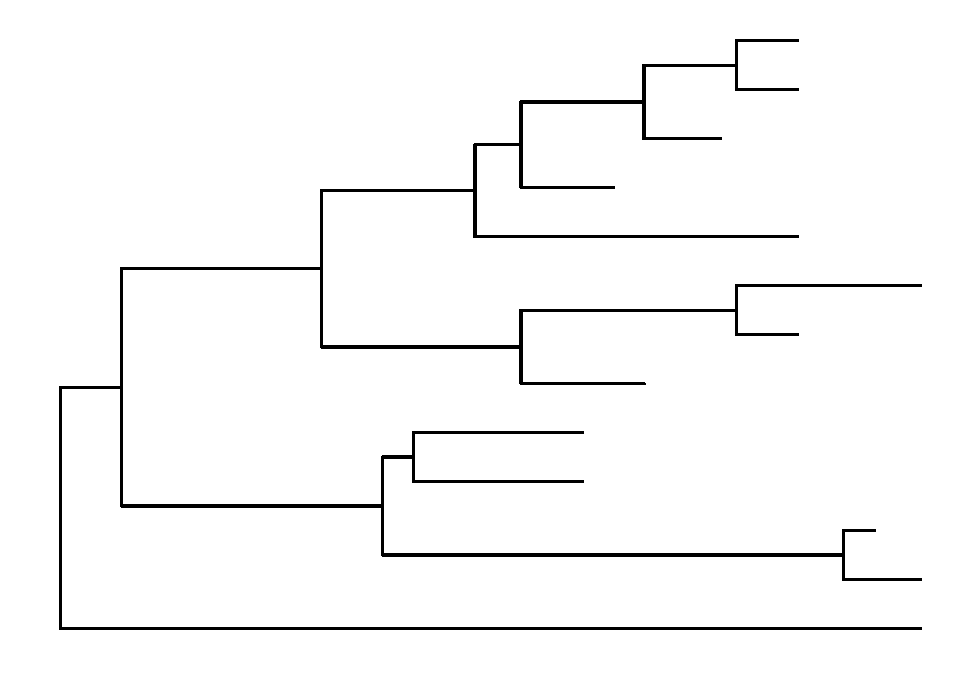
\includegraphics{ggtree_files/figure-latex/unnamed-chunk-8-1.pdf}

\subsubsection{themes}\label{themes}

\begin{Shaded}
\begin{Highlighting}[]
\KeywordTok{ggtree}\NormalTok{(}\KeywordTok{rtree}\NormalTok{(}\DecValTok{30}\NormalTok{), }\DataTypeTok{color=}\StringTok{"red"}\NormalTok{) }\OperatorTok{+}\StringTok{ }\KeywordTok{theme_tree}\NormalTok{(}\StringTok{"steelblue"}\NormalTok{)}
\end{Highlighting}
\end{Shaded}

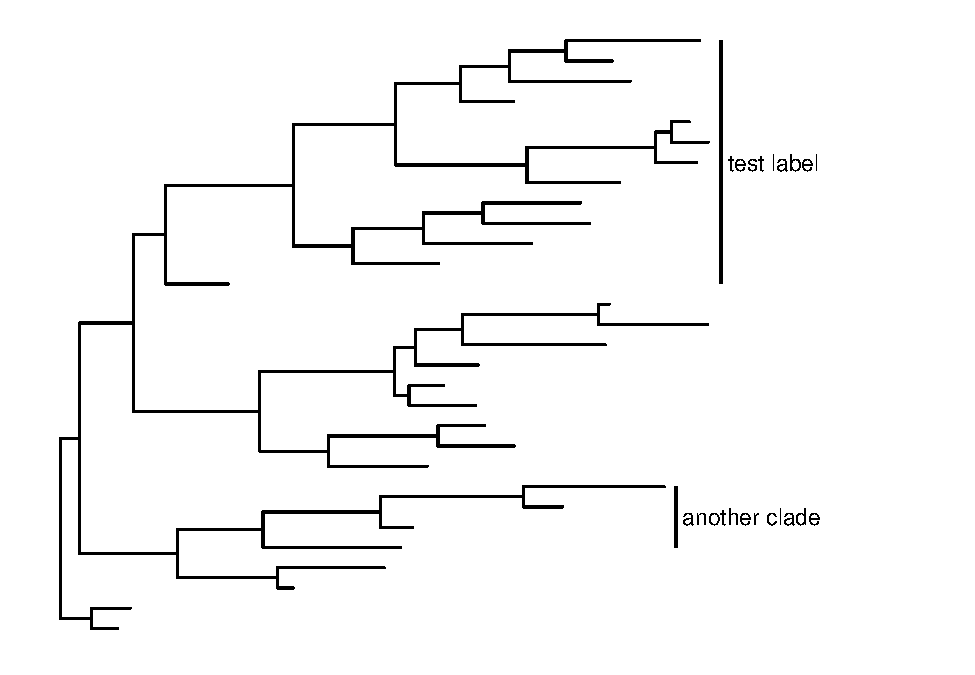
\includegraphics{ggtree_files/figure-latex/unnamed-chunk-9-1.pdf}

\begin{Shaded}
\begin{Highlighting}[]
\KeywordTok{ggtree}\NormalTok{(}\KeywordTok{rtree}\NormalTok{(}\DecValTok{20}\NormalTok{), }\DataTypeTok{color=}\StringTok{"white"}\NormalTok{) }\OperatorTok{+}\StringTok{ }\KeywordTok{theme_tree}\NormalTok{(}\StringTok{"black"}\NormalTok{)}
\end{Highlighting}
\end{Shaded}

\includegraphics{ggtree_files/figure-latex/unnamed-chunk-9-2.pdf}

\subsubsection{list of trees using multiPhylo; load ggplot2 for
facet\_wrap}\label{list-of-trees-using-multiphylo-load-ggplot2-for-facet_wrap}

\begin{Shaded}
\begin{Highlighting}[]
\NormalTok{trees <-}\StringTok{ }\KeywordTok{lapply}\NormalTok{(}\KeywordTok{c}\NormalTok{(}\DecValTok{10}\NormalTok{, }\DecValTok{20}\NormalTok{, }\DecValTok{40}\NormalTok{), rtree)}
\KeywordTok{class}\NormalTok{(trees) <-}\StringTok{ "multiPhylo"}
\KeywordTok{ggtree}\NormalTok{(trees) }\OperatorTok{+}\StringTok{ }\KeywordTok{facet_wrap}\NormalTok{(}\OperatorTok{~}\NormalTok{.id, }\DataTypeTok{scale=}\StringTok{"free"}\NormalTok{) }\OperatorTok{+}\StringTok{ }\KeywordTok{geom_tiplab}\NormalTok{()}
\end{Highlighting}
\end{Shaded}

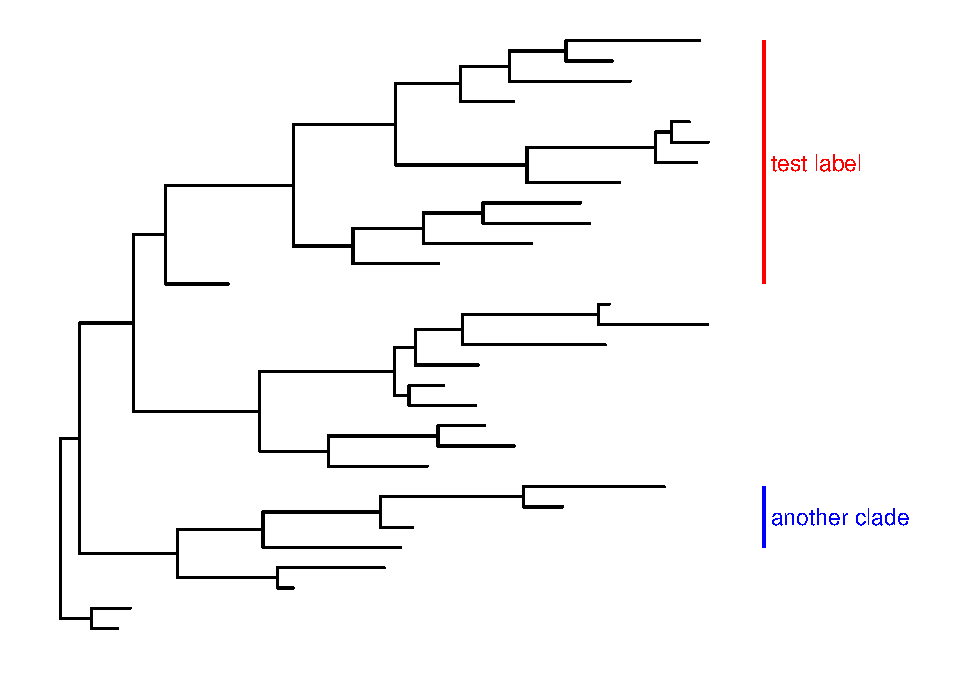
\includegraphics{ggtree_files/figure-latex/unnamed-chunk-10-1.pdf}

\subsubsection{zoom on a portion of a
tree}\label{zoom-on-a-portion-of-a-tree}

\begin{Shaded}
\begin{Highlighting}[]
\KeywordTok{library}\NormalTok{(}\StringTok{"ape"}\NormalTok{)}
\end{Highlighting}
\end{Shaded}

\begin{verbatim}
## 
## Attaching package: 'ape'
\end{verbatim}

\begin{verbatim}
## The following object is masked from 'package:ggtree':
## 
##     rotate
\end{verbatim}

\begin{Shaded}
\begin{Highlighting}[]
\KeywordTok{data}\NormalTok{(chiroptera)}
\KeywordTok{library}\NormalTok{(}\StringTok{"ggtree"}\NormalTok{)}
\KeywordTok{gzoom}\NormalTok{(chiroptera, }\KeywordTok{grep}\NormalTok{(}\StringTok{"Plecotus"}\NormalTok{, chiroptera}\OperatorTok{$}\NormalTok{tip.label))}
\end{Highlighting}
\end{Shaded}

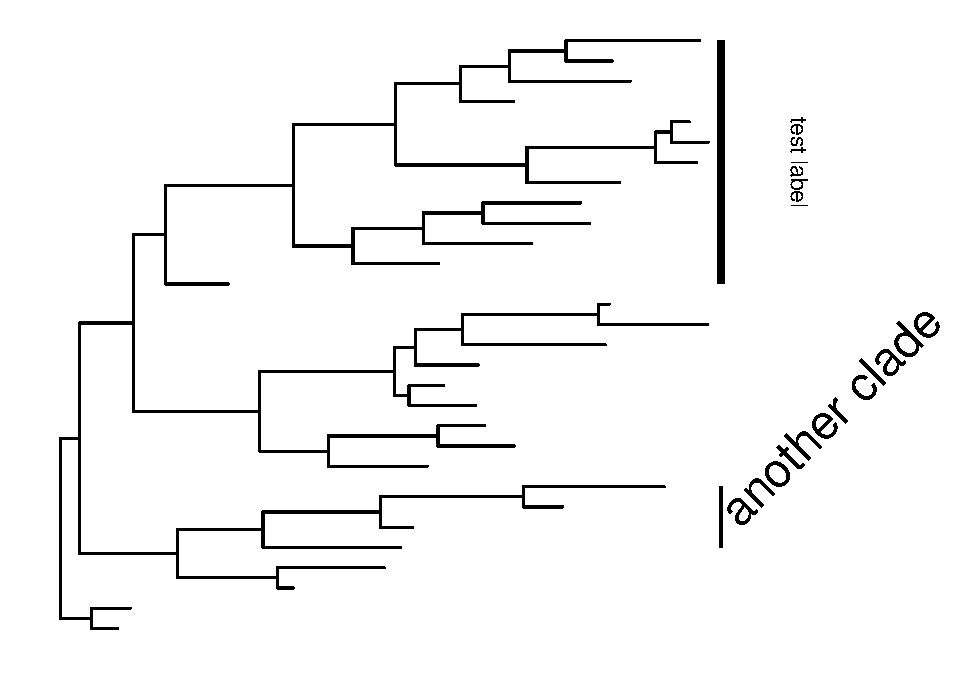
\includegraphics{ggtree_files/figure-latex/unnamed-chunk-11-1.pdf}

\subsection{TREE MANIPULATION}\label{tree-manipulation}

\begin{Shaded}
\begin{Highlighting}[]
\NormalTok{nwk <-}\StringTok{ }\KeywordTok{system.file}\NormalTok{(}\StringTok{"extdata"}\NormalTok{, }\StringTok{"sample.nwk"}\NormalTok{, }\DataTypeTok{package=}\StringTok{"treeio"}\NormalTok{)}
\NormalTok{tree <-}\StringTok{ }\KeywordTok{read.tree}\NormalTok{(nwk)}
\KeywordTok{ggtree}\NormalTok{(tree)}
\end{Highlighting}
\end{Shaded}

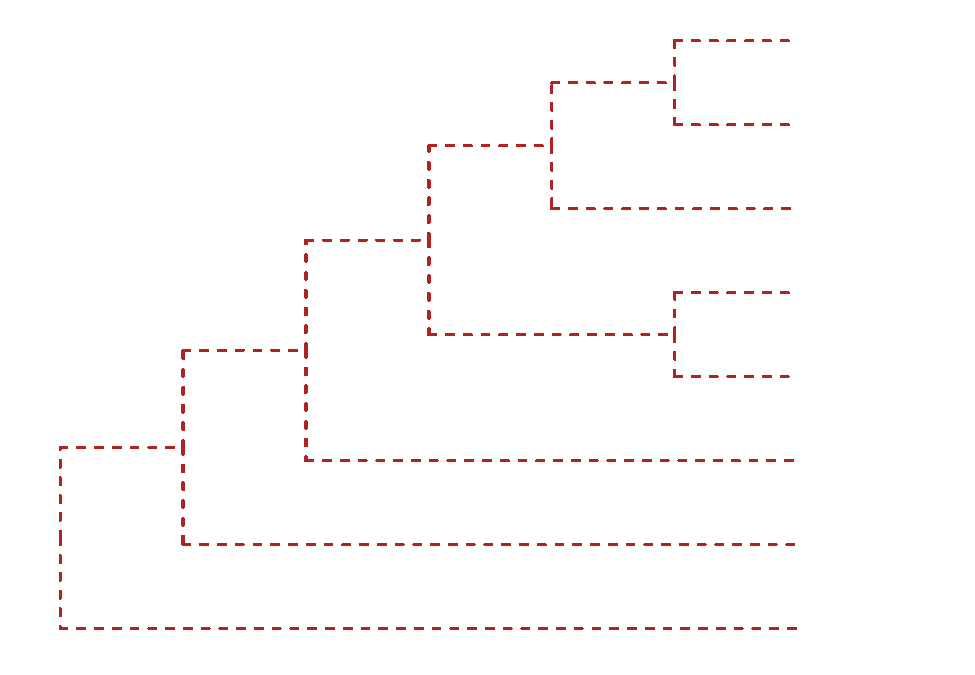
\includegraphics{ggtree_files/figure-latex/unnamed-chunk-12-1.pdf}

\begin{Shaded}
\begin{Highlighting}[]
\KeywordTok{ggtree}\NormalTok{(tree) }\OperatorTok{+}\StringTok{ }\KeywordTok{geom_text2}\NormalTok{(}\KeywordTok{aes}\NormalTok{(}\DataTypeTok{subset=}\OperatorTok{!}\NormalTok{isTip, }\DataTypeTok{label=}\NormalTok{node), }\DataTypeTok{hjust=}\OperatorTok{-}\NormalTok{.}\DecValTok{5}\NormalTok{) }\OperatorTok{+}\StringTok{ }\KeywordTok{geom_tiplab}\NormalTok{()}
\end{Highlighting}
\end{Shaded}

\includegraphics{ggtree_files/figure-latex/unnamed-chunk-12-2.pdf}

\subsubsection{View clade}\label{view-clade}

\begin{Shaded}
\begin{Highlighting}[]
\NormalTok{p <-}\StringTok{ }\KeywordTok{ggtree}\NormalTok{(tree)}
\KeywordTok{viewClade}\NormalTok{(p}\OperatorTok{+}\KeywordTok{geom_tiplab}\NormalTok{(), }\DataTypeTok{node=}\DecValTok{21}\NormalTok{)}
\end{Highlighting}
\end{Shaded}

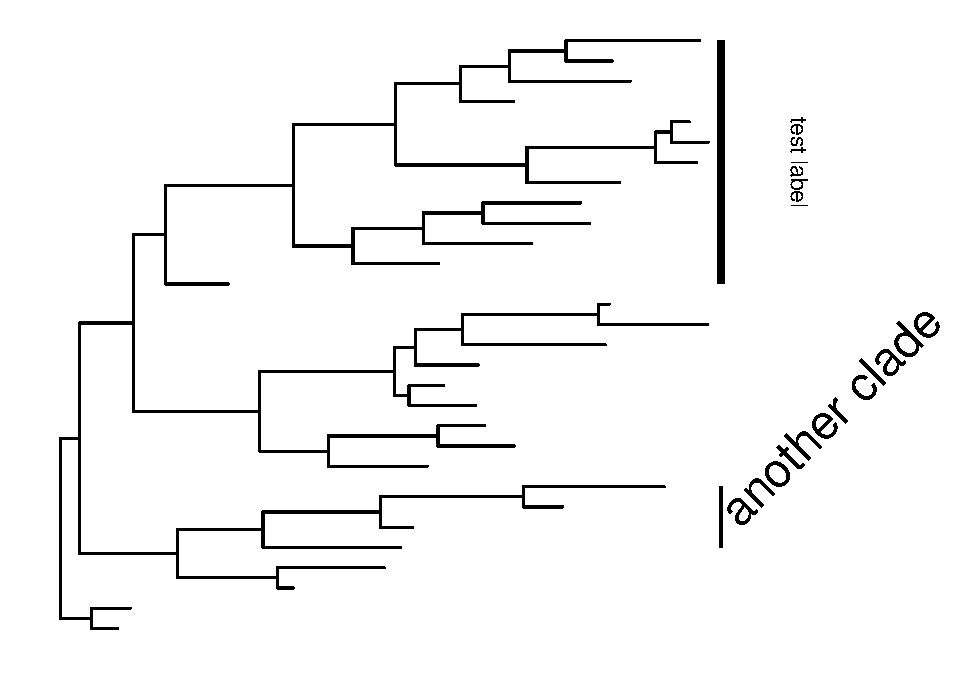
\includegraphics{ggtree_files/figure-latex/unnamed-chunk-13-1.pdf}

\subsubsection{Group clades}\label{group-clades}

use internal node or vector of internal nodes to cluster clades

\begin{Shaded}
\begin{Highlighting}[]
\NormalTok{tree <-}\StringTok{ }\KeywordTok{groupClade}\NormalTok{(tree, }\DataTypeTok{.node=}\DecValTok{21}\NormalTok{)}
\KeywordTok{ggtree}\NormalTok{(tree, }\KeywordTok{aes}\NormalTok{(}\DataTypeTok{color=}\NormalTok{group, }\DataTypeTok{linetype=}\NormalTok{group))}
\end{Highlighting}
\end{Shaded}

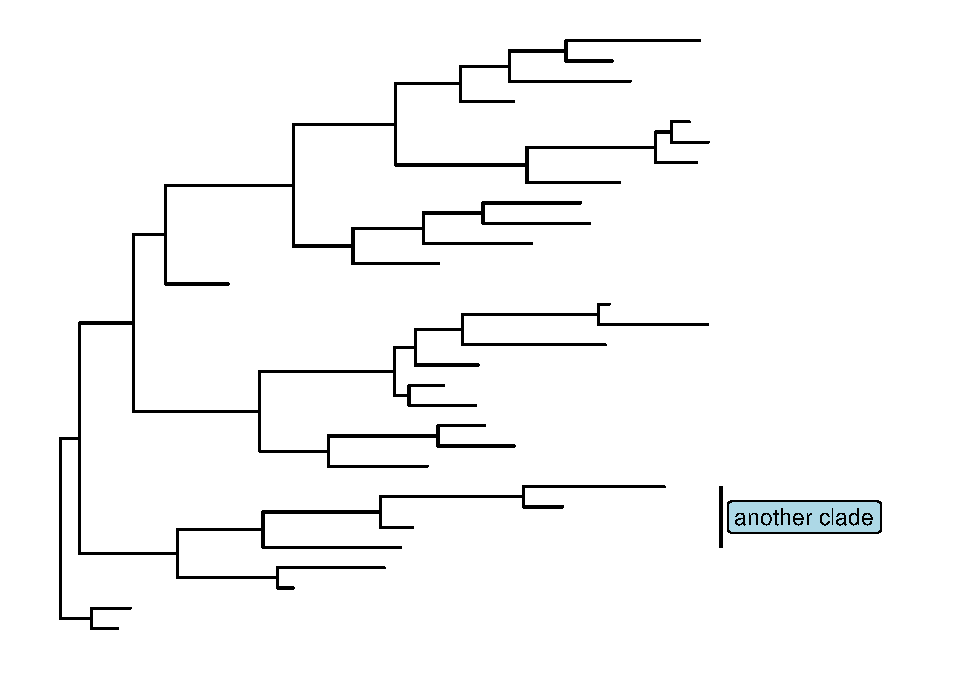
\includegraphics{ggtree_files/figure-latex/unnamed-chunk-14-1.pdf}

\begin{Shaded}
\begin{Highlighting}[]
\CommentTok{#ggtree(tree, aes(color=group, linetype=group)) + geom_text2(aes(label=node))}
\end{Highlighting}
\end{Shaded}

\subsubsection{Highlight selected taxa}\label{highlight-selected-taxa}

\begin{Shaded}
\begin{Highlighting}[]
\NormalTok{tree <-}\StringTok{ }\KeywordTok{groupClade}\NormalTok{(tree, }\DataTypeTok{.node=}\KeywordTok{c}\NormalTok{(}\DecValTok{21}\NormalTok{, }\DecValTok{17}\NormalTok{))}
\KeywordTok{ggtree}\NormalTok{(tree, }\KeywordTok{aes}\NormalTok{(}\DataTypeTok{color=}\NormalTok{group, }\DataTypeTok{linetype=}\NormalTok{group)) }\OperatorTok{+}\StringTok{ }\KeywordTok{geom_tiplab}\NormalTok{(}\KeywordTok{aes}\NormalTok{(}\DataTypeTok{subset=}\NormalTok{(group}\OperatorTok{==}\DecValTok{1}\NormalTok{)))}
\end{Highlighting}
\end{Shaded}

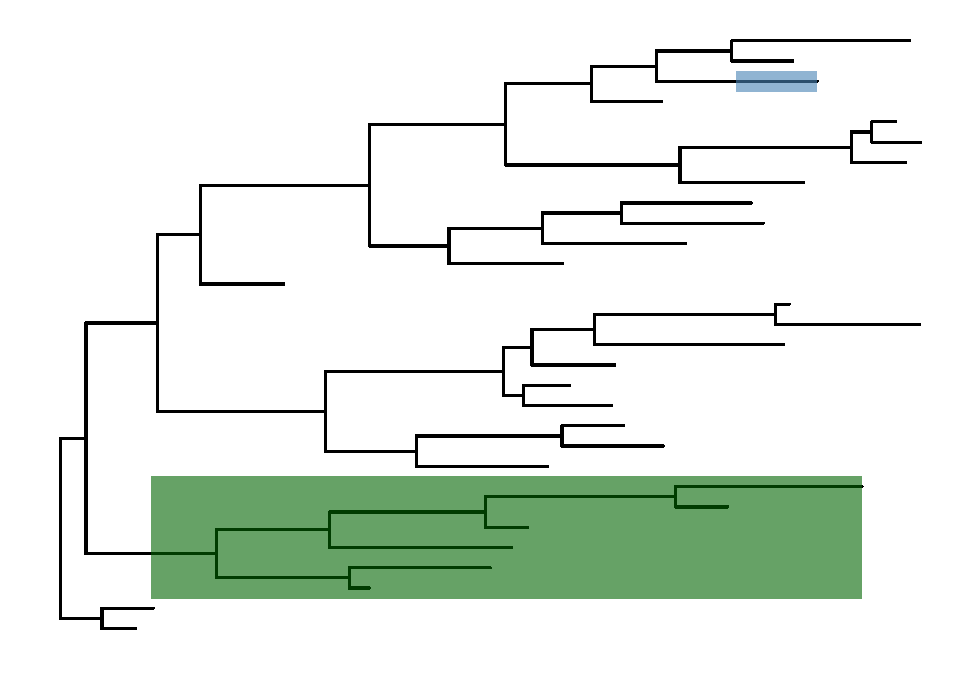
\includegraphics{ggtree_files/figure-latex/unnamed-chunk-15-1.pdf}

\begin{Shaded}
\begin{Highlighting}[]
\CommentTok{#ggtree(tree, aes(color=group, linetype=group)) + geom_tiplab(aes(subset=(group==2)))}
\CommentTok{# ggtree(tree, aes(color=group, linetype=group)) + geom_tiplab(aes(label=node))}
\end{Highlighting}
\end{Shaded}

\subsubsection{Collapse a clade}\label{collapse-a-clade}

\begin{Shaded}
\begin{Highlighting}[]
\NormalTok{cp <-}\StringTok{ }\KeywordTok{collapse}\NormalTok{(p, }\DataTypeTok{node=}\DecValTok{21}\NormalTok{)}
\NormalTok{cp }\OperatorTok{+}\StringTok{ }\KeywordTok{geom_point2}\NormalTok{(}\KeywordTok{aes}\NormalTok{(}\DataTypeTok{subset=}\NormalTok{(node }\OperatorTok{==}\StringTok{ }\DecValTok{21}\NormalTok{)), }\DataTypeTok{size=}\DecValTok{5}\NormalTok{, }\DataTypeTok{shape=}\DecValTok{23}\NormalTok{, }\DataTypeTok{fill=}\StringTok{"steelblue"}\NormalTok{)}
\end{Highlighting}
\end{Shaded}

\includegraphics{ggtree_files/figure-latex/unnamed-chunk-16-1.pdf}

\subsubsection{Expand collapsed clade}\label{expand-collapsed-clade}

\begin{Shaded}
\begin{Highlighting}[]
\NormalTok{cp }\OperatorTok\StringTok{ }\KeywordTok{expand}\NormalTok{(}\DataTypeTok{node=}\DecValTok{21}\NormalTok{)}
\end{Highlighting}
\end{Shaded}

\includegraphics{ggtree_files/figure-latex/unnamed-chunk-17-1.pdf}

\begin{Shaded}
\begin{Highlighting}[]
\NormalTok{p1 <-}\StringTok{ }\KeywordTok{ggtree}\NormalTok{(tree)}
\NormalTok{p2 <-}\StringTok{ }\KeywordTok{collapse}\NormalTok{(p1, }\DecValTok{21}\NormalTok{) }\OperatorTok{+}\StringTok{ }\KeywordTok{geom_point2}\NormalTok{(}\KeywordTok{aes}\NormalTok{(}\DataTypeTok{subset=}\NormalTok{(node}\OperatorTok{==}\DecValTok{21}\NormalTok{)), }\DataTypeTok{size=}\DecValTok{5}\NormalTok{, }\DataTypeTok{shape=}\DecValTok{23}\NormalTok{, }\DataTypeTok{fill=}\StringTok{"blue"}\NormalTok{)}
\NormalTok{p3 <-}\StringTok{ }\KeywordTok{collapse}\NormalTok{(p2, }\DecValTok{17}\NormalTok{) }\OperatorTok{+}\StringTok{ }\KeywordTok{geom_point2}\NormalTok{(}\KeywordTok{aes}\NormalTok{(}\DataTypeTok{subset=}\NormalTok{(node}\OperatorTok{==}\DecValTok{17}\NormalTok{)), }\DataTypeTok{size=}\DecValTok{5}\NormalTok{, }\DataTypeTok{shape=}\DecValTok{23}\NormalTok{, }\DataTypeTok{fill=}\StringTok{"red"}\NormalTok{)}
\NormalTok{p4 <-}\StringTok{ }\KeywordTok{expand}\NormalTok{(p3, }\DecValTok{17}\NormalTok{)}
\NormalTok{p5 <-}\StringTok{ }\KeywordTok{expand}\NormalTok{(p4, }\DecValTok{21}\NormalTok{)}

\KeywordTok{library}\NormalTok{(cowplot)}
\end{Highlighting}
\end{Shaded}

\begin{verbatim}
## 
## 
## *******************************************************
\end{verbatim}

\begin{verbatim}
## Note: cowplot does not change the default ggplot2 theme
\end{verbatim}

\begin{verbatim}
## anymore. To recover the previous behavior, execute:
##   theme_set(theme_cowplot())
\end{verbatim}

\begin{verbatim}
## *******************************************************
\end{verbatim}

\begin{Shaded}
\begin{Highlighting}[]
\KeywordTok{plot_grid}\NormalTok{(p1, p2, p3, p4, p5, }\DataTypeTok{ncol=}\DecValTok{5}\NormalTok{)}
\end{Highlighting}
\end{Shaded}

\includegraphics{ggtree_files/figure-latex/unnamed-chunk-18-1.pdf}

\subsubsection{Flip clades - should share a same
parent}\label{flip-clades---should-share-a-same-parent}

\begin{Shaded}
\begin{Highlighting}[]
\KeywordTok{plot_grid}\NormalTok{(p, }\KeywordTok{flip}\NormalTok{(p, }\DecValTok{17}\NormalTok{, }\DecValTok{21}\NormalTok{), }\DataTypeTok{ncol=}\DecValTok{2}\NormalTok{)}
\end{Highlighting}
\end{Shaded}

\includegraphics{ggtree_files/figure-latex/unnamed-chunk-19-1.pdf}

\subsubsection{Rotate a circular tree}\label{rotate-a-circular-tree}

\begin{Shaded}
\begin{Highlighting}[]
\ControlFlowTok{for}\NormalTok{ (angle }\ControlFlowTok{in} \KeywordTok{seq}\NormalTok{(}\DecValTok{0}\NormalTok{, }\DecValTok{270}\NormalTok{, }\DecValTok{30}\NormalTok{)) \{}
  \KeywordTok{print}\NormalTok{(}\KeywordTok{rotate_tree}\NormalTok{(p, angle) }\OperatorTok{+}\StringTok{ }\KeywordTok{ggtitle}\NormalTok{(}\KeywordTok{paste}\NormalTok{(}\StringTok{"rotate angle:"}\NormalTok{, angle)))}
\NormalTok{\}}
\end{Highlighting}
\end{Shaded}

\includegraphics{ggtree_files/figure-latex/unnamed-chunk-20-1.pdf}
\includegraphics{ggtree_files/figure-latex/unnamed-chunk-20-2.pdf}
\includegraphics{ggtree_files/figure-latex/unnamed-chunk-20-3.pdf}
\includegraphics{ggtree_files/figure-latex/unnamed-chunk-20-4.pdf}
\includegraphics{ggtree_files/figure-latex/unnamed-chunk-20-5.pdf}
\includegraphics{ggtree_files/figure-latex/unnamed-chunk-20-6.pdf}
\includegraphics{ggtree_files/figure-latex/unnamed-chunk-20-7.pdf}
\includegraphics{ggtree_files/figure-latex/unnamed-chunk-20-8.pdf}
\includegraphics{ggtree_files/figure-latex/unnamed-chunk-20-9.pdf}
\includegraphics{ggtree_files/figure-latex/unnamed-chunk-20-10.pdf}

\subsection{TREE ANNOTATION}\label{tree-annotation}

\subsubsection{Annotate a clade}\label{annotate-a-clade}

\begin{Shaded}
\begin{Highlighting}[]
\NormalTok{tree <-}\StringTok{ }\KeywordTok{rtree}\NormalTok{(}\DecValTok{30}\NormalTok{)}
\NormalTok{p <-}\StringTok{ }\KeywordTok{ggtree}\NormalTok{(tree) }\OperatorTok{+}\StringTok{ }\KeywordTok{xlim}\NormalTok{(}\OtherTok{NA}\NormalTok{, }\DecValTok{6}\NormalTok{)}
\CommentTok{#print(p) + geom_text2(aes(label=node))}
\NormalTok{p }\OperatorTok{+}\StringTok{ }\KeywordTok{geom_cladelabel}\NormalTok{(}\DataTypeTok{node=}\DecValTok{42}\NormalTok{, }\DataTypeTok{label=}\StringTok{"test label"}\NormalTok{) }\OperatorTok{+}
\StringTok{  }\KeywordTok{geom_cladelabel}\NormalTok{(}\DataTypeTok{node=}\DecValTok{55}\NormalTok{, }\DataTypeTok{label=}\StringTok{"another clade"}\NormalTok{)}
\end{Highlighting}
\end{Shaded}

\includegraphics{ggtree_files/figure-latex/unnamed-chunk-21-1.pdf}

\subsubsection{Adjust position}\label{adjust-position}

Use align = TRUE, to align the clade label, and use the parameter,
offset, to adjust the position.

\begin{Shaded}
\begin{Highlighting}[]
\NormalTok{p }\OperatorTok{+}\StringTok{ }\KeywordTok{geom_cladelabel}\NormalTok{(}\DataTypeTok{node=}\DecValTok{42}\NormalTok{, }\DataTypeTok{label=}\StringTok{"test label"}\NormalTok{, }\DataTypeTok{align=}\OtherTok{TRUE}\NormalTok{, }\DataTypeTok{offset=}\NormalTok{.}\DecValTok{3}\NormalTok{) }\OperatorTok{+}
\StringTok{  }\KeywordTok{geom_cladelabel}\NormalTok{(}\DataTypeTok{node=}\DecValTok{55}\NormalTok{, }\DataTypeTok{label=}\StringTok{"another clade"}\NormalTok{, }\DataTypeTok{align=}\OtherTok{TRUE}\NormalTok{, }\DataTypeTok{offset=}\NormalTok{.}\DecValTok{3}\NormalTok{)}
\end{Highlighting}
\end{Shaded}

\includegraphics{ggtree_files/figure-latex/unnamed-chunk-22-1.pdf}

\subsubsection{change color}\label{change-color}

\begin{Shaded}
\begin{Highlighting}[]
\NormalTok{p }\OperatorTok{+}\StringTok{ }\KeywordTok{geom_cladelabel}\NormalTok{(}\DataTypeTok{node=}\DecValTok{42}\NormalTok{, }\DataTypeTok{label=}\StringTok{"test label"}\NormalTok{, }\DataTypeTok{align=}\NormalTok{T, }\DataTypeTok{color=}\StringTok{'red'}\NormalTok{) }\OperatorTok{+}
\StringTok{  }\KeywordTok{geom_cladelabel}\NormalTok{(}\DataTypeTok{node=}\DecValTok{55}\NormalTok{, }\DataTypeTok{label=}\StringTok{"another clade"}\NormalTok{, }\DataTypeTok{align=}\NormalTok{T, }\DataTypeTok{color=}\StringTok{'blue'}\NormalTok{)}
\end{Highlighting}
\end{Shaded}

\includegraphics{ggtree_files/figure-latex/unnamed-chunk-23-1.pdf}

\subsubsection{change angle}\label{change-angle}

\begin{Shaded}
\begin{Highlighting}[]
\NormalTok{p }\OperatorTok{+}\StringTok{ }\KeywordTok{geom_cladelabel}\NormalTok{(}\DataTypeTok{node=}\DecValTok{42}\NormalTok{, }\DataTypeTok{label=}\StringTok{"test label"}\NormalTok{, }\DataTypeTok{align=}\NormalTok{T, }\DataTypeTok{angle=}\DecValTok{270}\NormalTok{, }\DataTypeTok{hjust=}\StringTok{'center'}\NormalTok{, }\DataTypeTok{offset.text=}\NormalTok{.}\DecValTok{5}\NormalTok{) }\OperatorTok{+}
\StringTok{  }\KeywordTok{geom_cladelabel}\NormalTok{(}\DataTypeTok{node=}\DecValTok{55}\NormalTok{, }\DataTypeTok{label=}\StringTok{"another clade"}\NormalTok{, }\DataTypeTok{align=}\NormalTok{T, }\DataTypeTok{angle=}\DecValTok{45}\NormalTok{)}
\end{Highlighting}
\end{Shaded}

\includegraphics{ggtree_files/figure-latex/unnamed-chunk-24-1.pdf}

\subsubsection{change the size of bar and
text}\label{change-the-size-of-bar-and-text}

\begin{Shaded}
\begin{Highlighting}[]
\NormalTok{p }\OperatorTok{+}\StringTok{ }\KeywordTok{geom_cladelabel}\NormalTok{(}\DataTypeTok{node=}\DecValTok{42}\NormalTok{, }\DataTypeTok{label=}\StringTok{"test label"}\NormalTok{, }\DataTypeTok{align=}\NormalTok{T, }\DataTypeTok{angle=}\DecValTok{270}\NormalTok{, }\DataTypeTok{hjust=}\StringTok{'center'}\NormalTok{, }\DataTypeTok{offset.text=}\NormalTok{.}\DecValTok{5}\NormalTok{, }\DataTypeTok{barsize=}\FloatTok{1.5}\NormalTok{) }\OperatorTok{+}
\StringTok{  }\KeywordTok{geom_cladelabel}\NormalTok{(}\DataTypeTok{node=}\DecValTok{55}\NormalTok{, }\DataTypeTok{label=}\StringTok{"another clade"}\NormalTok{, }\DataTypeTok{align=}\NormalTok{T, }\DataTypeTok{angle=}\DecValTok{45}\NormalTok{, }\DataTypeTok{fontsize=}\DecValTok{8}\NormalTok{)}
\end{Highlighting}
\end{Shaded}

\includegraphics{ggtree_files/figure-latex/unnamed-chunk-25-1.pdf}

\subsubsection{geom label can be used to label the
text}\label{geom-label-can-be-used-to-label-the-text}

\begin{Shaded}
\begin{Highlighting}[]
\NormalTok{p }\OperatorTok{+}\StringTok{ }\KeywordTok{geom_cladelabel}\NormalTok{(}\DataTypeTok{node=}\DecValTok{55}\NormalTok{, }\DataTypeTok{label=}\StringTok{"another clade"}\NormalTok{, }\DataTypeTok{align=}\NormalTok{T, }\DataTypeTok{geom=}\StringTok{'label'}\NormalTok{, }\DataTypeTok{fill=}\StringTok{'lightblue'}\NormalTok{)}
\end{Highlighting}
\end{Shaded}

\includegraphics{ggtree_files/figure-latex/unnamed-chunk-26-1.pdf}

\subsubsection{annotate clades for unrooted trees using
geom\_clade2}\label{annotate-clades-for-unrooted-trees-using-geom_clade2}

\begin{Shaded}
\begin{Highlighting}[]
\NormalTok{pg <-}\StringTok{ }\KeywordTok{ggtree}\NormalTok{(tree, }\DataTypeTok{layout=}\StringTok{"daylight"}\NormalTok{)}
\end{Highlighting}
\end{Shaded}

\begin{verbatim}
## Average angle change [1] 0.195496208341812
\end{verbatim}

\begin{verbatim}
## Average angle change [2] 0.0715680268737278
\end{verbatim}

\begin{verbatim}
## Average angle change [3] 0.0330818367838394
\end{verbatim}

\begin{Shaded}
\begin{Highlighting}[]
\NormalTok{pg }\OperatorTok{+}\StringTok{ }\KeywordTok{geom_cladelabel2}\NormalTok{(}\DataTypeTok{node=}\DecValTok{42}\NormalTok{, }\DataTypeTok{label=}\StringTok{"test label"}\NormalTok{, }\DataTypeTok{angle=}\DecValTok{10}\NormalTok{) }\OperatorTok{+}
\StringTok{  }\KeywordTok{geom_cladelabel2}\NormalTok{(}\DataTypeTok{node=}\DecValTok{55}\NormalTok{, }\DataTypeTok{label=}\StringTok{"another clade"}\NormalTok{, }\DataTypeTok{angle=}\DecValTok{305}\NormalTok{)}
\end{Highlighting}
\end{Shaded}

\includegraphics{ggtree_files/figure-latex/unnamed-chunk-27-1.pdf}

\subsubsection{Highlight clades}\label{highlight-clades}

\begin{Shaded}
\begin{Highlighting}[]
\KeywordTok{ggtree}\NormalTok{(tree) }\OperatorTok{+}\StringTok{ }\KeywordTok{geom_hilight}\NormalTok{(}\DataTypeTok{node=}\DecValTok{21}\NormalTok{, }\DataTypeTok{fill=}\StringTok{"steelblue"}\NormalTok{, }\DataTypeTok{alpha=}\NormalTok{.}\DecValTok{6}\NormalTok{) }\OperatorTok{+}
\StringTok{  }\KeywordTok{geom_hilight}\NormalTok{(}\DataTypeTok{node=}\DecValTok{54}\NormalTok{, }\DataTypeTok{fill=}\StringTok{"darkgreen"}\NormalTok{, }\DataTypeTok{alpha=}\NormalTok{.}\DecValTok{6}\NormalTok{)}
\end{Highlighting}
\end{Shaded}

\includegraphics{ggtree_files/figure-latex/unnamed-chunk-28-1.pdf}

For more details on ggtree, please refer to the webiste
{[}\url{http://bioconductor.org/packages/release/bioc/html/ggtree.html}{]}

\subsection{THANK YOU}\label{thank-you}


\end{document}
